\documentclass[11pt,a4paper,oldfontcommands]{memoir}
\usepackage{ctex}
\usepackage[utf8]{inputenc}
\usepackage[T1]{fontenc}
\usepackage{microtype}
\usepackage[dvips]{graphicx}
\usepackage{xcolor}
\definecolor{linkColor}{RGB}{0, 153, 230}

\usepackage{times}
\usepackage{listings}
\usepackage{courier}
\lstset{
    columns=fixed,       
    numbers=left,                                                          % 在左侧显示行号
    frame=none,                                                            % 不显示背景边框
    backgroundcolor=\color[RGB]{245,245,244},            % 设定背景颜色
    keywordstyle=\color[RGB]{40,40,255},                      % 设定关键字颜色
    numberstyle=\footnotesize\color{darkgray},             % 设定行号格式
    commentstyle=\color[RGB]{0,96,96},                        % 设置代码注释的格式
    stringstyle=\rmfamily\slshape\color[RGB]{128,0,0},   % 设置字符串格式
    showstringspaces=false,                                           % 不显示字符串中的空格
    language=c++,                                                        % 设置语言
    basicstyle=\small\ttfamily
}

\usepackage[
breaklinks=true,colorlinks=true,
%linkcolor=blue,urlcolor=blue,citecolor=blue,% PDF VIEW
linkcolor=black,urlcolor=black,citecolor=black,% PRINT
bookmarks=true,bookmarksopenlevel=2]{hyperref}

\usepackage{amsmath}
\usepackage{hyperref}

\usepackage{geometry}
% PDF VIEW
% \geometry{total={210mm,297mm},
% left=25mm,right=25mm,%
% bindingoffset=0mm, top=25mm,bottom=25mm}
% PRINT
\geometry{total={210mm,297mm},
left=20mm,right=20mm,
bindingoffset=10mm, top=25mm,bottom=25mm}

\OnehalfSpacing
\chapterstyle{bianchi}
\setsecheadstyle{\Large\bfseries\sffamily\raggedright}
\setsubsecheadstyle{\large\bfseries\sffamily\raggedright}
\setsubsubsecheadstyle{\bfseries\sffamily\raggedright}

\pagestyle{plain}
\makepagestyle{plain}
\makeevenfoot{plain}{\thepage}{}{}
\makeoddfoot{plain}{}{}{\thepage}
\makeevenhead{plain}{}{}{}
\makeoddhead{plain}{}{}{}
\maxsecnumdepth{subsection} % chapters, sections, and subsections are numbered
\maxtocdepth{subsection} % chapters, sections, and subsections are in the Table of Contents

\graphicspath{ {./figure/} }

\begin{document}
\thispagestyle{empty}
{
\sffamily
\centering
{\LARGE
Introduction To 3D Game Programming with DirectX12 笔记
}

\vspace{3.5cm}
(草稿)\\
翻译参考\\
\href{http://shiba.hpe.sh.cn/jiaoyanzu/WULI/Soft/NotXNA}{\textcolor{linkColor}{DirecX11 学习笔记}}\\
Google 翻译
\clearpage
\tableofcontents*
\clearpage
\chapter{向量代数(Vector Algebra)}
\chapter{矩阵代数(Matrix Algebra)}
\chapter{矩阵变换(Transformation)}
\chapter{Direct3D 初始化(Direct3D Initialization)}

\chapter{渲染管道(The Rendering Pipeline)}
\section{3D图像(The 3D Illusion)}
\section{模型表达(Model Representation)}
\section{基本计算颜色(Basic Computer Color)}
\begin{flushleft}
计算机显示器在每个像素发射一种混合红、绿、蓝三种颜色的光。当这种混合光到达眼睛并且击中视网膜区域,视锥细胞收到刺激并将产生的神经冲动通过视觉神经传递到大脑。大脑解释这种信号为颜色。随着混合光的变化,使这些视锥细胞收到不同的刺激,从而使大脑中产生不同的颜色。
\end{flushleft}

\subsection{颜色运算(Color Operations)}
\begin{itemize}
    \item 加法:$(0.0, 0.5, 0) + (0, 0.0, 0.25) = (0.0, 0.5, 0.25)$
    \item 减法:$(1, 1, 1) - (1, 1, 0) = (0, 0, 1)$
    \item 标量乘法:$0.5(1, 1, 1) = (0.5, 0.5, 0.5)$
    \item 显然,点乘和叉乘对于颜色向量来说没有意义。然而,颜色向量有一特殊的运算称为调制或分量乘法:$(c_{r},c_{g},c_{b}) \otimes (k_{r},k_{g},k_{b}) = (c_{r}k_{r},c_{g}k_{g},c_{b}k_{b})$。该运算主要用来作为照明方程。举个例子,假设我们有一束入射光线(r,g,b),它会照射一个反射50%红光,75%绿光和25%蓝光的表面,并吸收剩余的光线。 然后反射光线的颜色由下式给出:$(r,g,b) \otimes (0.5,0.75,0.25) = (0.5r,0.75g,0.25b)$
\end{itemize}

\subsection{128位颜色(128-Bit Color)}
\begin{flushleft}
通常我们会合并另外的颜色分量,称作 alpha 分量。alpha 分量常用来表示颜色的透明度(透明度在混合中很有用,因为我们还没有使用混合,目前只需将 alpha 分量设为 1 即可)。包含 alpha 分量意味着我们用 4D 颜色向量$(r, g, b, a), 0 \leq r,g,b,a \leq 1$ 为了用 128-bits 表示一种颜色,每个分量使用浮点型值。因为数学上,一种颜色就是一个 4D 向量,我们能在代码中使用 XMVECTOR 类型来表示一种颜色,并且每当调用 DirectX Math 中的向量函数时都会受益于 SIMD (如,颜色加减和标量乘法)。为了方便分量乘法,DirectX Math 库提供了下面方法:
\begin{lstlisting}
// Return c1 \otimes c2
XMVECTOR XM_CALLCONV XMColorModulate(FXMVECTOR C1, FXMVECTOR C2);
\end{lstlisting}
\end{flushleft}

\subsection{32位颜色(32-Bit Color)}
\begin{flushleft}
要以32位大小来表示一个颜色,可以给每个分量分配一个字节(8-bit)大小。这样一来,每个分量最多能表现256种色调——0代表无强度,255代表满强度,中间值代表中间强度。看似每个分量一个字节很小,但是组合在一起$(256 \times 256 \times 256)$就表示百万种不同的颜色。DirectX Math 库(\#include <DirectXPackedVector.h>) DirectX::PackedVector 命名空间(namespace)下提供了以下数据结构来存储32位颜色:
\begin{lstlisting}
namespace DirectX
{
namespace PackedVector
{
    // ARGB Color; 8-8-8-8 bit unsigned normalized integer components packed
    // into a 32 bit integer. The normalized color is packed into 32 bits
    // using 8 bit unsigned, normalized integers for the alpha, red, green,
    // and blue components.
    // The alpha component is stored in the most significant bits and the
    // blue component in the least significant bits (A8R8G8B8):
    // [32] aaaaaaaa rrrrrrrr gggggggg bbbbbbbb [0]
    struct XMCOLOR
    {
        union
        {
            struct
            {
                uint8_t b; // Blue: 0/255 to 255/255
                uint8_t g; // Green: 0/255 to 255/255
                uint8_t r; // Red: 0/255 to 255/255
                uint8_t a; // Alpha: 0/255 to 255/255
            };
            uint32_t c;
        };
        XMCOLOR() {}
        XMCOLOR(uint32_t Color) : c(Color) {}
        XMCOLOR(float _r, float _g, float _b, float _a);
        explicit XMCOLOR(_In_reads_(4) const float *pArray);
        operator uint32_t () const { return c; }
        XMCOLOR& operator= (const XMCOLOR& Color) 
        { c = Color.c; return *this; }
        XMCOLOR& operator= (const uint32_t Color) 
        { c = Color; return *this; }
    };
} // end PackedVector namespace
} // end DirectX namespace
\end{lstlisting}
一个32位颜色数据能被转换为128位颜色数据: 将整数区间$[0, 255]$ 映射到实数区间$[0, 1]$。每个数除以255即可,也就是说 设$0 \leq n \leq 255$,且 n 是整数,则 $0 \leq \frac{n}{255} \leq 1$ 就是需要的范围 0 到 1 的颜色强度。例:(80,140,200,255)转换如下:
$$ (80,140,200,255)\rightarrow (\frac{80}{255},\frac{140}{255},\frac{200}{255},\frac{255}{255}) \approx (0.31,0.55,0.78,1.0)$$
另一方面,128位颜色能转换为32位颜色:将每个分量乘以255并且四舍五入取整。例:
$$(0.3,0.6,0.9,1.0)\rightarrow (0.3\cdot 255,0.6\cdot 255,0.9\cdot 255,1.0\cdot 255)=(77,153,230,255)$$

在将32位颜色转换为128位颜色时通常必须执行额外的位操作,反之,因为8位颜色组件通常打包为32位整数值(如 unsigned int),XMCOLOR 就是如此。DirectXMath 库定义了一个方法以 XMCOLOR 作为参数,返回XMVECTOR:
\begin{lstlisting}
XMVECTOR XM_CALLCONV PackedVector::XMLoadColor(const XMCOLOR* pSource);
\end{lstlisting}
\end{flushleft}

\section{渲染管道概览(Overview of the rendering pipeline)}
\section{输入汇编程序阶段(The Input Assembler Stage)}
\subsection{顶点(Vertices)}
\subsection{原始拓扑(Primitive Topology)}
\subsection{指数(Indices)}
\section{顶点着色器阶段(The Vertex Shader Stage)}
\subsection{局部空间和世界空间(Local Space and World Space)}
TODO
\subsection{视图空间(View Space)}
\begin{flushleft}
为了形成场景的二维图像,我们必须在场景中放置一个虚拟相机。 相机指定了观众可以看到的世界的多大的体积,以及我们需要生成多大的世界体积来生成二维图像。让我们将一个局部坐标系统(称为视图空间,眼图空间或相机空间)附加到相机,如图\ref{fig:5-19}所示; 也就是说,摄像机坐落在正视z轴的原点处,x轴指向摄像机的右侧,y轴指向摄像机的上方。 而不是描述相对于世界空间的场景顶点,基于相机坐标系,渲染管线的后面阶段很方便地描述它们。从世界空间到视图空间的坐标变换称为视图变换,相应的矩阵称为视图矩阵。\\
\begin{figure}[t]
    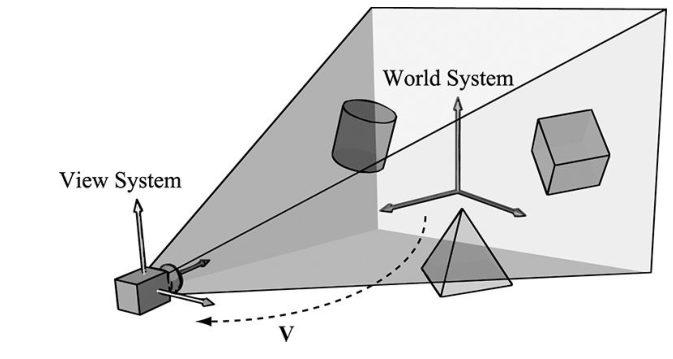
\includegraphics[width=\textwidth]{5-19}
    \centering
    \caption{转换顶点相对于世界空间的坐标,使它们相对于相机空间。}
    \label{fig:5-19}
\end{figure}
如果$Q_{w}=(Q_{x},Q_{y},Q_{z},1)$,$u_{w}=(u_{x},u_{y},u_{z},0)$,$v_{w}=(v_{x},v_{y},v_{z},0)$,$w_{w}=(w_{x},w_{y},w_{z},0)$分别用相对于世界空间的齐次坐标来描述视图空间的原点,x轴,y轴和z轴,然后我们从3.4.3一节知道坐标矩阵从视图空间的变化到世界空间是:
$$W=
\begin{bmatrix}
u_{x} & u_{y} & u_{z} & 0\\
v_{x} & v_{y} & v_{z} & 0\\
w_{x} & w_{y} & w_{z} & 0\\
Q_{x} & Q_{y} & Q_{z} & 1
\end{bmatrix}$$\\
然而,这不是我们想要的转换。我们想要的是倒置转换,即从世界空间转换成视图空间。回忆3.4.3节,倒置转换就是求矩阵的逆。因此$W^{-1}$就是从世界空间到视图空间的转换。\\
世界坐标系统和视图坐标系统仅在位置和方向有区别,所以直观地得到 $W=RT$(也就是说世界矩阵能被分解为一个旋转跟一个平移(translation))\footnote{$R$是\href{https://en.wikipedia.org/wiki/Orthogonal_matrix}{\textcolor{linkColor}{正交矩阵}},所以有 $R^{-1}=R^{T}$}。这让求逆变得简单:
\begin{align*}
V&=W^{-1}=(RT)^{-1}=T^{-1}R^{-1}=T^{-1}R^{T} \\
&=\begin{bmatrix}
1 & 0 & 0 & 0\\
0 & 1 & 0 & 0\\
0 & 0 & 1 & 0\\
-Q_{x} & -Q_{y} & -Q_{z} & 1
\end{bmatrix}
\begin{bmatrix}
u_{x} & v_{x} & w_{x} & 0\\
u_{y} & v_{y} & w_{y} & 0\\
u_{z} & v_{z} & w_{z} & 0\\
0 & 0 & 0 & 0
\end{bmatrix} \\
&=\begin{bmatrix}
u_{x} & v_{x} & w_{x} & 0\\
u_{y} & v_{y} & w_{y} & 0\\
u_{z} & v_{z} & w_{z} & 0\\
\mathbf{-Q\cdot u} & \mathbf{-Q\cdot v} & \mathbf{-Q\cdot w} & 1
\end{bmatrix}
\end{align*}

所以,视图矩阵就是:
\begin{align*}
V=\begin{bmatrix}
u_{x} & v_{x} & w_{x} & 0\\
u_{y} & v_{y} & w_{y} & 0\\
u_{z} & v_{z} & w_{z} & 0\\
\mathbf{-Q\cdot u} & \mathbf{-Q\cdot v} & \mathbf{-Q\cdot w} & 1
\end{bmatrix}
\end{align*}
现在我们用一种直观的方式来构造向量,这些向量用来建立视图矩阵。令\textbf{Q}为摄像机的位置,\textbf{T}为摄像机对准的目标点。然后,令\textbf{j}为世界空间向上方向的单位向量。(本书中,世界坐标系的 xz 构成的平面作为世界地平面,世界 y 轴描述了向上的方向;所以,$j=(0,1,0)$ 就是和世界 y 轴平行的单位向量。然而这只是约定,一些应用可能会选择 xy构成的平面作为地平面,z轴作为向上方向。)参考图片\ref{fig:5-20},摄像机的朝向如下:
$$w=\frac{T-Q}{||T-Q||}$$
该向量描述的是摄像机的z轴,对准\textbf{w}右侧的单位向量:\\
$$u=\frac{j\times w}{||j \times w||}$$
该向量描述的是摄像机的 x 轴。最后,摄像机的y轴单位向量为:\\
$$v=w \times u$$
因为\textbf{w}和\textbf{u}是互相正交的单位向量,$w\times u$也必定是单位向量,没必要正规化。\\
综上所述,给定摄像机的位置,目标点,和世界向上方向,我们就能求得摄像机的本地坐标系统,作为视图矩阵。
\begin{figure}[t]
    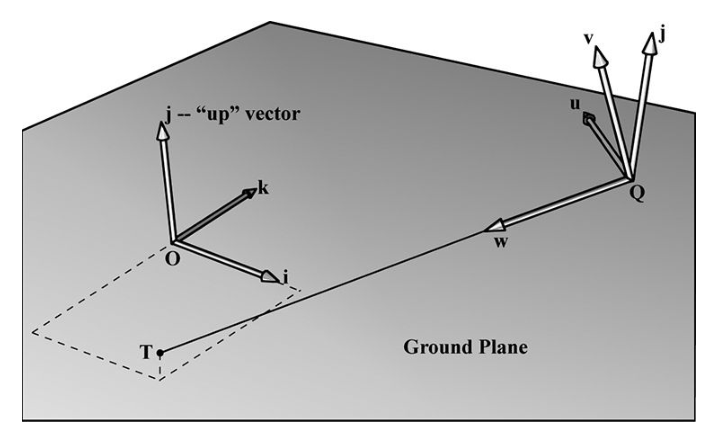
\includegraphics[width=\textwidth]{5-20}
    \centering
    \caption{根据相机位置,目标点和世界“向上”矢量构造相机坐标系。}
    \label{fig:5-20}
\end{figure}

DirectXMath 库提供了计算视图矩阵的方法:
\begin{lstlisting}
// Outputs view matrix V
XMVECTOR XM_CALLCONV XMMatrixLookAtLH(
    FXMVECTOR EyePosition,    // Input camera position Q
    FXMVECTOR FocusPosition,  // Input target point T
    FXMVECTOR UpDirection);   // Input world up direction j
\end{lstlisting}
通常世界y轴就是向上的方向,所以$j=(0,1,0)$ 就是向上的向量。例:假设我们将摄像机放在相对于世界坐标的$(5,3,-10)$处,并且对准世界原点坐标$(0,0,0)$。可以通过下面方式获得视图矩阵:\\
\begin{lstlisting}
XMVECTOR pos    = XMVectorSet(5, 3, -10, 1.0f);
XMVECTOR target = XMVectorZero();
XMVECTOR up     = XMVectorSet(0.0f, 1.0f, 0.0f, 0.0f);
XMMATRIX V      = XMMatrixLookAtLH(pos, target, up);
\end{lstlisting}
\end{flushleft}
\subsection{投影和齐次裁剪空间(Projection and Homogeneous Clip Space)}
\begin{flushleft}
到目前为止我们描述了在世界空间中摄像机的位置和方向,但摄像机还有一个部分需要解决,即摄像机看到的空间体积。体积由视锥来描述(见图\ref{fig:5-21})。
\end{flushleft}
\begin{figure}[t]
    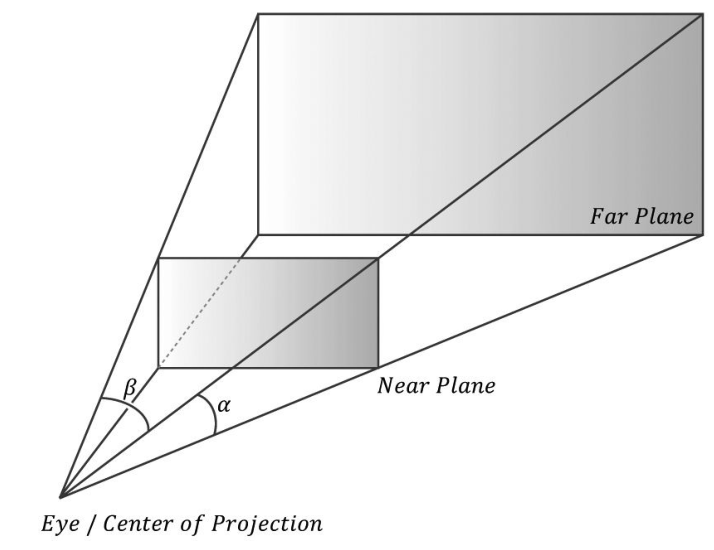
\includegraphics[width=\textwidth]{5-21}
    \centering
    \caption{视锥定义了摄像机“看到”的空间体积}
    \label{fig:5-21}
\end{figure}
\begin{flushleft}
我们接下来的任务是将一个 3D 几何体在视锥中投影到 2D 投影窗口中。投影必须以平行线汇聚到消失点的方式完成,当一个物体的3D深度增加(距离拉远),投影的大小就减小。这就是\href{https://en.wikipedia.org/wiki/Perspective_(graphical)}{\textcolor{linkColor}{透视投影}}(如图\ref{fig:5-22})。我们将一个顶点到视点(眼睛所在的位置,姑且叫视点吧)的连线称为顶点的投影线。然后我们定义透视投影变换就是3D顶点\textbf{v}变换成它的投影线和2D投影面板交叉点\textbf{v'}的过程;我们认为\textbf{v'}就是\textbf{v}的投影。一个3D物体的投影就是组成这个物体的所有顶点的投影。
\end{flushleft}
\begin{figure}[t]
    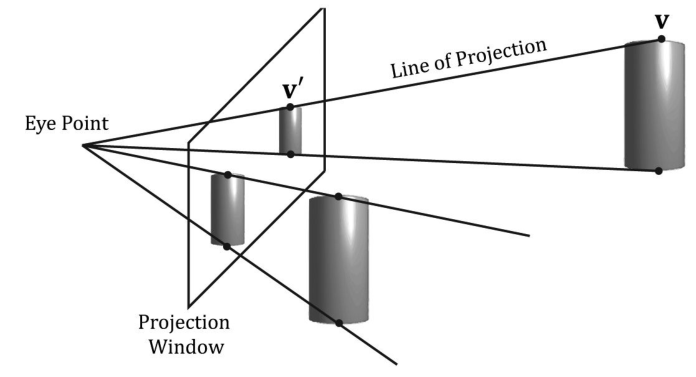
\includegraphics[width=\textwidth]{5-22}
    \centering
    \caption{两个圆柱体大小相同,但深度不同。距离眼睛近的圆柱体比距离远的圆柱体投影大。视锥中的几何体被投影到投影窗口;视锥外的集合体,投影到投影面板上,但在投影窗口外面(投影面板和投影窗口共面)}
    \label{fig:5-22}
\end{figure}

\paragraph{定义一个视锥(Defining a Frustum)}
\begin{flushleft}
我们可以在视图空间中定义一个视锥,其投影中心位于原点处,并沿着正z轴向下看,通过以下四个量:近平面$n$,远平面$f$,垂直视场角$\alpha$ 和纵横比 $r$。请注意,在视图空间中,近平面和远平面平行于$xy$平面; 因此我们只需指定它们沿着z轴的原点距离。 纵横比由 $r=w/h$ 定义,其中$w$是投影窗口的宽度,$h$是投影窗口的高度(视图空间中的单位)。 投影窗口本质上是视图空间中场景的二维图像。 这里的图像最终将映射到后台缓冲区(back buffer); 因此,我们喜欢投影窗口尺寸的比率与后台缓冲区尺寸的比率相同。所以后缓冲区维度的比率通常被指定为长宽比(这是一个比例,所以它没有单位)。例,如果后台缓冲区尺寸是 $800 \times 600$,则 $r=\frac{800}{600} \approx 1.333$。如果投影窗口与后台缓冲区的纵横比不相同,则需要非均匀缩放来将投影窗口映射到后台缓冲区,这将导致失真(例如,投影窗口上的圆圈可能当映射到后台缓冲区时被拉伸成一个椭圆)。\\
我们将水平视角标记为$\beta$,垂直视角标记为$\alpha$,纵横比为$r$。要看看$r$如何帮助我们找到$\beta$,请考虑图\ref{fig:5-23}。 请注意,投影窗口的实际尺寸并不重要,只需要保持纵横比。 因此,我们会选择2的方便高度,因此宽度必须为:\\
$$r=\frac{w}{h}=\frac{w}{2}\Rightarrow w=2r$$
\end{flushleft}
\begin{figure}[t]
    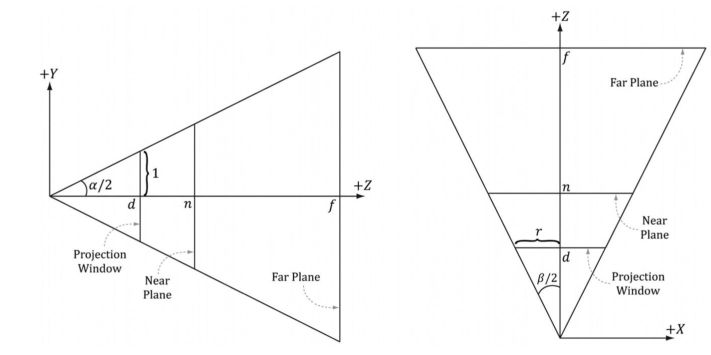
\includegraphics[width=\textwidth]{5-23}
    \centering
    \caption{给定垂直视角$\alpha$和纵横比$r$,得出水平视角$\beta$}
    \label{fig:5-23}
\end{figure}
\begin{flushleft}
为了具有指定的垂直视场$\alpha$,投影窗口必须放置在距离原点的距离$d$处:
$$\tan(\frac{\alpha}{2})=\frac{1}{d}\Rightarrow d=\cot(\frac{\alpha}{2})$$
现在我们已经将投影窗沿$z$轴的距离d固定为当投影窗的高度为2时垂直视场$\alpha$。现在我们可以求解$\beta$。 看一下图\ref{fig:5-23}中的$xz$平面,我们现在看到:
$$\tan(\frac{\beta}{2})=\frac{r}{d}=\frac{r}{\cot(\frac{\alpha}{2})}=r\cdot \tan(\frac{\alpha}{2})$$
因此,考虑到垂直视角α和纵横比r,我们总能得到水平视角β:
$$\beta=2\tan^{-1}(r\cdot\tan(\frac{\alpha}{2}))$$
\end{flushleft}

\paragraph{投影顶点(Projecting Vertices)}
\begin{figure}[t]
    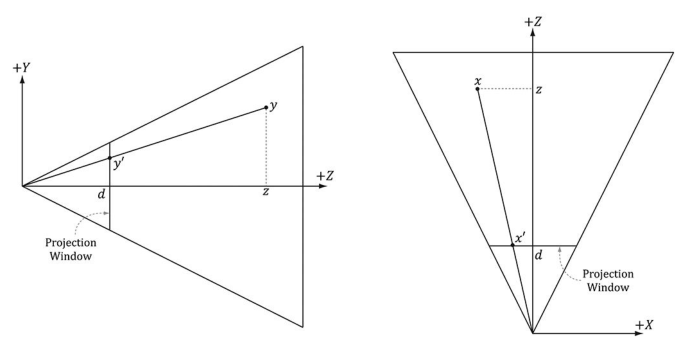
\includegraphics[width=\textwidth]{5-24}
    \centering
    \caption{相似三角}
    \label{fig:5-24}
\end{figure}
\begin{flushleft}
参考图\ref{fig:5-24}。 给定一个点$(x,y,z)$,我们希望在投影平面$z = d$上找到它的投影$(x',y',d)$。 通过分别考虑$x$和$y$坐标并使用相似的三角形,我们发现:
\begin{align*}
\frac{x'}{d}=\frac{x}{z}\Rightarrow x'=\frac{xd}{z}=\frac{x\cot(\alpha/2)}{z}=\frac{x}{z\tan(\alpha/2)}\\
\frac{y'}{d}=\frac{y}{z}\Rightarrow y'=\frac{yd}{z}=\frac{y\cot(\alpha/2)}{z}=\frac{y}{z\tan(\alpha/2)}\\
\end{align*}
显然对于点$(x,y,z)$, $-r\leq x'\leq r,-1\leq y'\leq 1,n\leq z\leq f$
\end{flushleft}

\paragraph{标准化的设备坐标(Normalized Device Coordinate-NDC)}
\begin{flushleft}
上一节中投影点的坐标是在视图空间中计算的。 在视图空间中,投影窗口的高度为2,宽度为$2r$,其中$r$是纵横比。 问题在于,尺寸取决于宽高比。 这意味着我们需要告诉硬件高宽比,因为硬件稍后需要做一些涉及投影窗口尺寸的操作(比如将其映射到后台缓冲区)。 如果我们能够消除这种对长宽比的依赖性会更方便。 解决的办法是将投影的$x$坐标从区间$[-r,r]$缩放到$[-1,1]$像这样:
\begin{align*}
-r\leq x' \leq r \\
-1\leq x'/r \leq 1
\end{align*}

在映射之后,$x$坐标和$y$坐标被称为标准化的设备坐标(NDC)(z坐标还没有被标准化),并且点$(x,y,z)$在视锥内当且仅当:
\begin{align*}
-1\leq x'/r \leq 1 \\
-1\leq y' \leq 1 \\
n \leq z \leq f
\end{align*}

从视图空间到NDC空间的转换可视为单位转换。 我们有一个关系,即一个NDC单位在$x$轴上等于视图空间中的$r$个单位(即 1ndc = \textbf{r} vs)。 所以给定$x$个视图空间单位,我们可以使用这个关系来转换单位:
$$x\mathit{vs}\cdot \frac{1\mathit{ndc}}{r\mathit{vs}}=\frac{x}{r}\mathit{ndc}$$
我们可以修改我们的投影公式,直接在NDC坐标中为我们提供投影的$x$坐标和$y$坐标:
\begin{align*}\tag{eq.5.1}\label{eq.5.1}
x'&=\frac{x}{rz\tan(\alpha/2)}\\
y'&=\frac{y}{z\tan(\alpha/2)}
\end{align*}
请注意,在NDC坐标中,投影窗口的高度为2,宽度为2.因此,现在尺寸是固定的,硬件无需知道纵横比,但我们有责任始终在NDC中提供投影坐标空间(图形硬件假设我们会)。
\end{flushleft}

\paragraph{用矩阵来描述投影公式(Writing the Projection Equations with a Matrix)}
\begin{flushleft}
为了保持一致,我们将用一个矩阵来描述投影变换。不过,公式\ref{eq.5.1}是非线性的,无法用矩阵描述。所以我们要使用一种“技巧”将它分为两部分来实现:一个线性部分和一个非线性部分。非线性部分要除以$z$。我们会在下一节讨论“如何规范化$z$坐标”时讲解这一问题;现在读者只需要知道,我们会因为个除法操作而失去原始的z坐标。所以,我们必须在变换之前保存输入的z坐标;我们可以利用齐次坐标来解决一问题,将输入的$z$坐标复制给输出的$w$坐标。在矩阵乘法中,我们要将元素[2][3]设为1、元素[3][3]设为0(从0开始的索引)。我们的投影矩阵大致如下:
\begin{align*}
P=\begin{bmatrix}
\frac{1}{r\tan(\alpha/2)} & 0 & 0 & 0\\
0 & \frac{1}{\tan(\alpha/2)} & 0 & 0\\
0 & 0 & A & 1\\
0 & 0 & B & 0
\end{bmatrix}
\end{align*}
注意矩阵中的常量$A$和$B$(它们将在下一节讨论);这些常量用于把输入的$z$坐标变换到规范化区间。将一个任意点$(x,y,z,1)$与该矩阵相乘,可以得到:
\begin{align*}\tag{eq.5.2}\label{eq.5.2}
[x,y,z,1]\begin{bmatrix}
\frac{1}{r\tan(\alpha/2)} & 0 & 0 & 0\\
0 & \frac{1}{\tan(\alpha/2)} & 0 & 0\\
0 & 0 & A & 1\\
0 & 0 & B & 0
\end{bmatrix}=\left[ \frac{x}{r\tan(\alpha/2)},\frac{y}{\tan(\alpha/2)},Az+B,z\right]
\end{align*}
在与投影矩阵(线性部分)相乘之后,我们要将每个坐标除以$w = z$(非线性部分),得到最终的变换结果:
\begin{align*}\tag{eq.5.3}\label{eq.5.3}
\left[ \frac{x}{r\tan(\alpha/2)},\frac{y}{\tan(\alpha/2)},Az+B,z\right]
\xrightarrow[]{\text{除以$w$}}
\left[ \frac{x}{rz\tan(\alpha/2)},\frac{y}{z\tan(\alpha/2)},A+\frac{B}{z},1\right]
\end{align*}
顺便提一句,你可能会问:“如何处理除数为0的情况”;对于一问题我们不必担心,因为近平面总是大于0的,其他的点都会被裁剪掉(参见5.9节)。有时,与$w$相除的过程也称为透视除法(perspective divide)或齐次除法(homogeneous divide)。我们可以看到$x$、$y$的投影坐标与公式\ref{eq.5.1}相同。
\end{flushleft}

\paragraph{规范化深度值}
\begin{flushleft}
你可能认为在投影之后可以丢弃原始的3D $z$坐标,因为所有的投影点已经摆放在2D投影窗口上,形成了我们最终看到的2D图像,不会再使用3D $z$坐标了。其实不然,我们仍然需要为深度缓存算法提供3D深度信息。就如同Direct3D希望我们把$x$、$y$投影坐标映射到一个规范化区间一样,Direct3D也希望我们将深度坐标映射到一个规范化区间$[0,1]$中。所以,我们需要创建一个保序函数(order preserving function)$g(x)$把$[n,f]$区间映射到$[0,1]$区间。由于该函数是保序的,所以当$z_{1},z_{2}∈[n,f]$且$z_{1}<z_{2}$时,必有$g(z_{1})<g(z_{2})$。这样,即使深度值已经被变换过了,相对的深度关系还是会被完好无损地保留下来,我们依然可以在规范化区间中得到正确的深度测试结果,这就是我们要为深度缓存算法做的全部工作。
通过缩放和平移可以实现从$[n ,f]$到$[0,1]$的映射。但是,这种方式无法与我们当前的投影方程整合。我们可以从公式\ref{eq.5.3}中看到经过变换的$z$坐标为:
$$g(z)=A+\frac{B}{z}$$
我们现在需要让$A$和$B$满足以下条件:
\begin{itemize}
    \item 条件1:$g(n)=A+\frac{B}{n}$(近平面映射为0)
    \item 条件2:$g(f)=A+\frac{B}{f}$(远平面映射为1)
\end{itemize}
由条件1得到$B$的结果为:$B=-An$。把它代入条件2,得到$A$的结果为:
\begin{align*}
A+\frac{-An}{f}=1\\
\frac{Af-An}{f}=1\\
Af-An=f\\
A=\frac{f}{f-n}
\end{align*}
所以:
\begin{align*}
g(z)=\frac{f}{f-n}-\frac{nf}{(f-n)z}
\end{align*}
从$g(z)$的曲线图(图\ref{fig:5-25})中可以看出,它会限制增长的幅度(保序)而且是非线性的。从图中我们还可以看到,区间中的大部分取值落在近平面附近。因此,大多数深度值被映射到了一个很窄的取值范围内。这会导致深度缓冲区出现精度问题(由于所能表示的数值范围有限,计算机将无法识别变换后的深度值之间的微小差异)。通常的建议是让近平面和远平面尽可能接近,把深度的精度性问题减小到最低程度。
\end{flushleft}
\begin{figure}[b]
    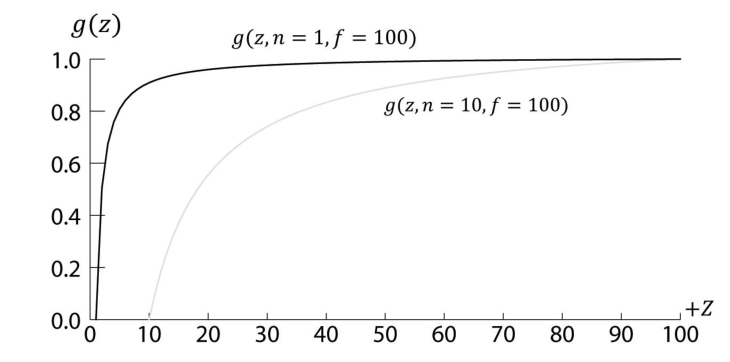
\includegraphics[width=\textwidth]{5-25}
    \centering
    \caption{相对于不同近平面的$g(z)$曲线图}
    \label{fig:5-25}
\end{figure}
\begin{flushleft}
现在我们已经解出了A和B,我们可以确定出完整的透视投影矩阵:
\begin{align*}
P=\begin{bmatrix}
\frac{1}{r\tan(\alpha/2)} & 0 & 0 & 0\\
0 & \frac{1}{\tan(\alpha/2)} & 0 & 0\\
0 & 0 & \frac{f}{f-n} & 1\\
0 & 0 & \frac{-nf}{f-n} & 0
\end{bmatrix}
\end{align*}
在与投影矩阵相乘之后,进行透视除法之前,几何体所处的空间称为齐次裁剪空间(homogeneous clip space)或投影空间(projection space)。在透视除法之后,几何体所处的空间称为规范化设备空间(normalized device coordinates,简称NDC)。
\end{flushleft}

\paragraph{XMMatrixPerspectiveFovLH}
\begin{flushleft}
一个透视投影矩阵能由下面的 DirectX Math 函数生成:
\begin{lstlisting}
// Return the projection matrix
XMMATRIX XM_CALLCONV XMMatrixPerspectiveFovLH(
    float FovAngleY, // vertical field of view angle in radians
    float Aspecct,     // aspect ratio = width / height
    float NearZ,       // distance to near plane
    float FarZ);         // distance to far plane
\end{lstlisting}
下面代码展示了如何使用 XMMatrixPerspectiveFovLH。这里,我们定义垂直视角为$45^{\circ}$,近平面$z=1$,远平面$z=1000$(这些长度都在视图空间)
\begin{lstlisting}
XMMATRIX P= XMMatrixPerspectiveFovLH(0.25f*XM_PI, AspectRatio(),1.0f,1000.0f);
\end{lstlisting}
纵横比匹配窗口的纵横比:
\begin{lstlisting}
float D3DApp::AspectRatio() const
{
  return static_cast<float>(mClientWidth) / mClientHeight;
}
\end{lstlisting}
\end{flushleft}

\section{镶嵌阶段(曲面细分阶段)(The Tessellation Stages)}
\begin{flushleft}
镶嵌(Tessellation)是指通过添加三角形的方式对一个网格的三角形进行细分,这些新添加的三角形可以偏移到一个新的位置,让网格的细节更加丰富。如图\ref{fig:5-26}
\end{flushleft}
\begin{figure}[h]
    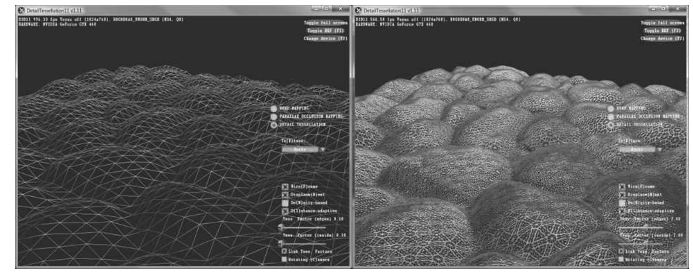
\includegraphics[width=\textwidth]{5-26}
    \centering
    \caption{左图是原网格,右图是镶嵌后的网格}
    \label{fig:5-26}
\end{figure}

\begin{flushleft}
下面是曲面细分的好处:
\begin{itemize}
    \item 我们可以实现细节层次(level-of-detail, LOD),使靠近相机的三角形通过细分产生更多细节,而那些远离相机的三角形则保持不变。通过这种方式,我们只需在需要细节的地方使用更多的三角形就可以了。
    \item 我们可以在内存中保存一个低细节(低细节意味着三角形数量少)的网格,但可以实时地添加额外的三角形,这样可以节省内存。
    \item 我们可以在一个低细节的网格上处理动画和物理效果,而只在渲染时才使用细分过的高细节网格。
\end{itemize}
曲面细分阶段是Direct3D 11中新添加的,这样我们就可以在GPU上对几何体进行细分了。而在Direct3D 11之前,如果你想要实现曲面细分,则必须在CPU上完成,经过细分的几何体还要发送到GPU用于渲染。然而,将新的几何体从CPU内存发送到显存是很慢的,而且还会增加CPU的负担。因此,在Direct3D 11出现之前,曲面细分的方法在实时图形中并不流行。Direct3D 11提供了一个可以完全在硬件上实现的曲面细分API。这样曲面细分就成为了一个非常有吸引力的技术了。曲面细分阶段是可选的(即在需要的时候才使用它)。我们要在第14章才会详细介绍曲面细分。
\end{flushleft}

\section{几何着色阶段(The Geometry Shader Stage)}
\begin{flushleft}
几何着色器阶段(geometry shader stage)是可选的,我们在第12章之前不会用到它,所以这里只做一个简短的概述。几何着色器以完整的图元作为输入数据。例如,当我们绘制三角形列表时,输入到几何着色器的数据是构成三角形的三个点。(注意,这三个点是从顶点着色器传递过来的。)几何着色器的主要优势是它可以创建或销毁几何体。例如,输入图元可以被扩展为一个或多个其他图元,或者几何着色器可以根据某些条件拒绝输出某些图元。这一点与顶点着色器有明显的不同:顶点着色器无法创建顶点,只要输入一个顶点,那么就必须输出一个顶点。几何着色器通常用于将一个点扩展为一个四边形,或者将一条线扩展为一个四边形。\\
~\\
我们可以在图5.11中看到一个“流输出(stream output)”箭头。也就是,几何着色器可以将顶点数据流输出到内存中的一个顶点缓冲区内,这些顶点可以在管线的随后阶段中渲染出来。这是一项高级技术,我们会在后面的章节中对它进行讨论。\\
~\\
NOTICE:顶点位置在离开几何着色器之前,必须被变换到齐次裁剪空间。
\end{flushleft}

\section{裁剪(Clipping)}
\begin{flushleft}
我们必须完全丢弃在平截头体之外的几何体,裁剪与平截头体边界相交的几何体,只留下平截头体内的部分;图 \ref{fig:5-27}以2D形式说明了一概念。
\begin{figure}[h]
    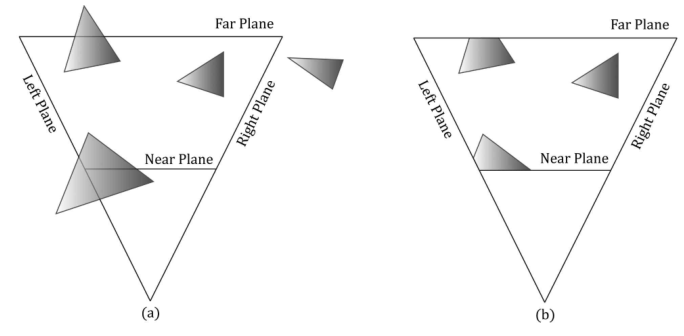
\includegraphics[width=\textwidth]{5-27}
    \centering
    \caption{(a)裁剪之前,(b)裁剪之后}
    \label{fig:5-27}
\end{figure}
我们可以将平截头体视为由6个平面界定的空间范围:顶、底、左、右、近、远平面。要裁剪与平截头体方向相反的多边形,其实就是逐个裁剪与每个平截头体平面方向相反的多边形,当裁剪一个与平面方向相反的多边形时(参见图\ref{fig:5-28}),我们将保留平面正半空间中的部分,而丢弃平面负半空间中的部分。对一个与平面方向相反的凸多边形进行裁剪,得到的结果仍然会是一个凸多边形。由于硬件会自动完成所有的裁剪工作,所以我们不在这里讲解具体的实现细节;有兴趣的读者可以参阅[Sutherland74],了解一下目前流行的Sutherland-Hodgeman裁剪算法。它基本思路是:求出平面与多边形边之间的交点,然后对顶点进行排序,形成新的裁剪后的多边形。\\
\begin{figure}[h]
    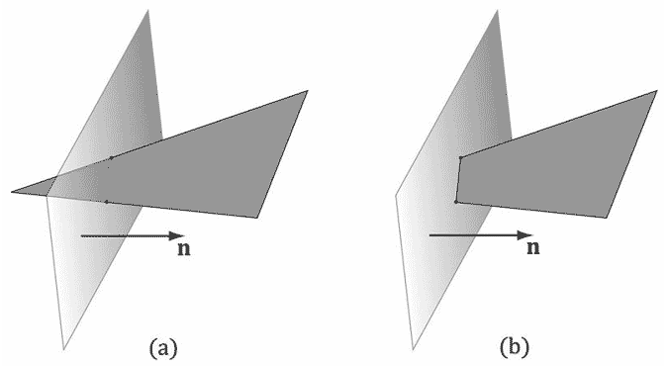
\includegraphics[width=\textwidth]{5-28}
    \centering
    \caption{(a)裁剪一个与平面方向相反的三角形,(b)裁剪后的三角形。注意,裁剪后的三角形已经不再是一个三角形了,它是一个四边形。所以,硬件必须将这个四边形重新划分为三角形,对于凸多边形来说这是一个非常简单的处理过程。}
    \label{fig:5-28}
\end{figure}
\begin{figure}[h]
    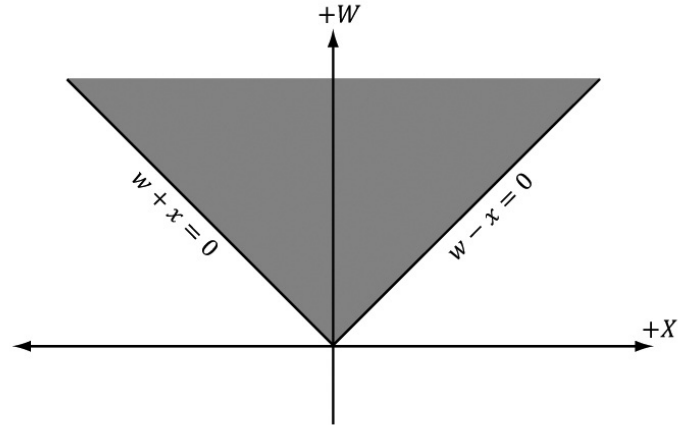
\includegraphics[width=\textwidth]{5-29}
    \centering
    \caption{齐次裁剪空间中$xw$平面上的截头体边界}
    \label{fig:5-29}
\end{figure}
[Blinn78]描述了如何在4D齐次空间中实现裁剪算法(图\ref{fig:5-29})。在透视除法之后,平截头体内的点$ (\frac{x}{w},\frac{y}{w},\frac{z}{w},1) $将位于规范化设备空间,它的边界如下:
\begin{align*}
-1\leq x/w \leq 1\\
-1\leq y/w \leq 1\\
0 \leq z/w \leq 1
\end{align*}
那么在透视除法之前,平截头体内的4D点(x , y , z , w)在齐次裁剪空间中的边界为:
\begin{align*}
-w\leq x \leq w\\
-w\leq y \leq w\\
0 \leq z \leq w
\end{align*}
也就是,顶点被限定在以下4D平面构成的空间范围内:
\begin{align*}
\mathit{Left:}&w=-x\\
\mathit{Right:}&w=x\\
\mathit{Bottom:}&w=-y\\
\mathit{Top:}&w=y\\
\mathit{Near:}&z=0\\
\mathit{Far:}&z=w
\end{align*}
只要我们知道齐次剪裁空间中的平截头体平面方程,我们就能使用任何一种裁剪算法(比如Sutherland-Hodgeman)。注意,由线段/平面相交测试的数学推论可知,这个测试在$\mathbf{R}^{4}$也能使用,所以我们可以在齐次裁剪空间中进行4D点和4D平面的相交测试。
\end{flushleft}

\section{光栅化阶段(The Rasterization Stage)}
\begin{flushleft}
光栅化(rasterization)阶段的主要任务是为投影后的3D三角形计算像素颜色。
\end{flushleft}
\subsection{视口变换(Viewport Transform)}
\begin{flushleft}
在裁剪之后,硬件会自动执行透视除法,将顶点从齐次裁剪空间变换到规范化设备空间(NDC)。一旦顶点进入NDC空间,构成2D图像的2D x、y坐标就会被变换到后台缓冲区中的一个称为视口的矩形区域内(回顾4.2.8节)。在该变换之后,$x$、$y$坐标将以像素为单位。通常,视口变换不修改$z$坐标,因为z坐标还要由深度缓存使用,但是我们可以通过 D3D12\_VIEWPORT 结构体的 MinDepth 和 MaxDepth 值修改z坐标的取值范围。MinDepth 和 MaxDepth 的值必须在0和1之间。
\end{flushleft}
\subsection{背面剔除(Backface Culling)}
\begin{flushleft}
一个三角形有两个面。我们使用如下约定来区分这两个面。假设三角形的顶点按照$v_{0}$、$v_{1}$、$v_{2}$的顺序排列,我们这样来计算三角形的法线$n$:
\begin{align*}
e_{0}&=v_{1}-v_{0}\\
e_{1}&=v_{2}-v_{1}\\
n&=\frac{e_{0}\times e_{1}}{||e_{0}\times e_{1}||}
\end{align*}
带有法线向量的面为正面,而另一个面为背面。图\ref{fig:5-30}说明了这一概念。
\begin{figure}[h]
    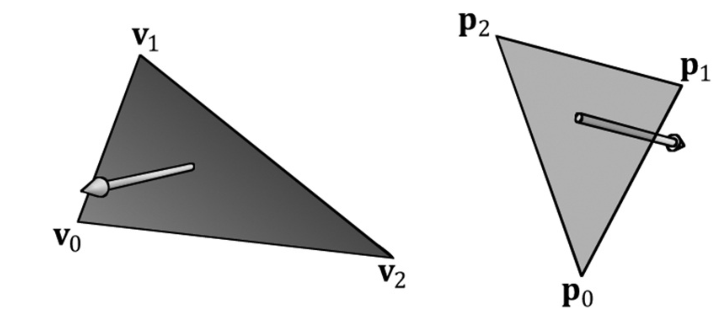
\includegraphics[width=\textwidth]{5-30}
    \centering
    \caption{左边的三角形正对我们的观察点,而右边的三角形背对我们的观察点。}
    \label{fig:5-30}
\end{figure}
当观察者看到三角形的正面时,我们说三角形是朝前的;当观察者看到三角形的背面时, 我们说三角形是朝后的。如图\ref{fig:5-30}所示,左边的三角形是朝前的,而右边的三角形是朝后的。而且,按照我们的观察角度,左边的三角形会按顺时针方向环绕,而右边的三角形会按逆时针方向环绕。这不是巧合:因为按照我们选择的约定(即,我们计算三角形法线的方式),按顺时针方向环绕的三角形(相对于观察者)是朝前的,而按逆时针方向环绕的三角形(相对于观察者)是朝后的。\\
~\\
现在,3D空间中的大部分物体都是封闭实心物体。当我们按照这一方式将每个三角形的法线指向物体外侧时,摄像机就不会看到实心物体朝后的三角形,因为朝前的三角形挡住了朝后的三角形;图\ref{fig:5-31}和图\ref{fig:5-32}分别以2D和3D形式说明了一概念。由于朝前的三角形挡住了朝后的三角形,所以绘制它们是毫无意义的。背面消隐(backface culling)是指让管线放弃对朝后的三角形的处理。这可以将所要处理的三角形的数量降低到原数量的一半。
\end{flushleft}
\begin{figure}[h]
    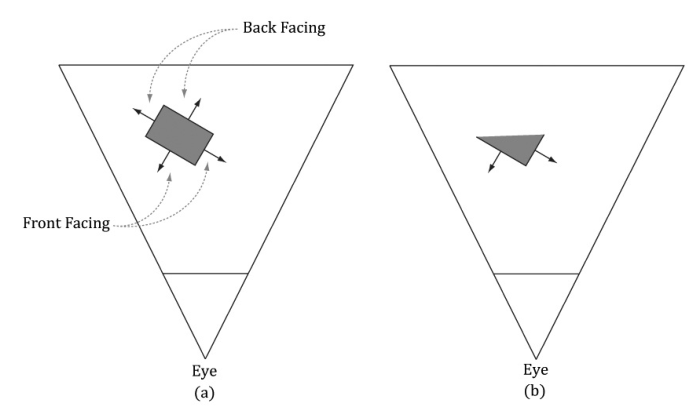
\includegraphics[width=\textwidth]{5-31}
    \centering
    \caption{(a)一个带有朝前和朝后三角形的实心物体。(b)在剔除了朝后的三角形之后的场景。注意,背面消隐不会影响最终的图像,因为朝后的三角形会被朝前的三角形阻挡。}
    \label{fig:5-31}
\end{figure}
\begin{figure}[h]
    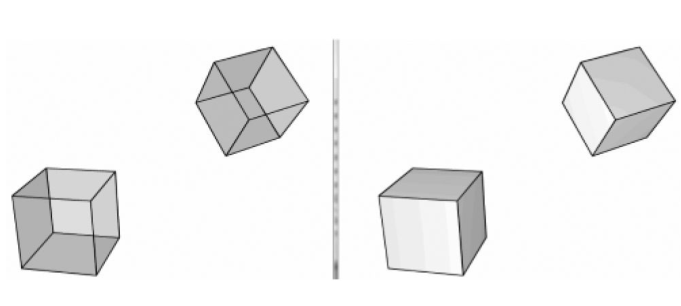
\includegraphics[width=\textwidth]{5-32}
    \centering
    \caption{(左图)当以透明方式绘制立方体时,我们可以看到所有的6个面。(右图)当以实心方式绘制立方体时,我们无法看到朝后的3个面,因为朝前的3个面挡住了它们——所以朝后的三角形可以被直接丢弃,不再接受后续处理,没人能看到些朝后的三角形。}
    \label{fig:5-32}
\end{figure}
\begin{flushleft}
默认情况下,Direct3D将(相对于观察者)顺时针方向环绕的三角形视为朝前的三角形,将(相对于观察者)逆时针方向环绕的三角形视为朝后的三角形。不过,这一约定可以通过修改Direct3D渲染状态颠倒过来。
\end{flushleft}

\subsection{顶点属性插值(Vertex Attribute Interpolation)}
\begin{flushleft}
如前所述,我们通过指定三角形的3个顶点来定义一个三角形。除位置外,顶点还可以包含其他属性,比如颜色、法线向量和纹理坐标。在视口变换之后,这些属性必须为三角形表面上的每个像素进行插值。顶点深度值也必须进行插值,以使每个像素都有一个可用于深度缓存算法的深度值。对屏幕空间中的顶点属性进行插值,其实就是对3D空间中的三角形表面进行线性插值(如图\ref{fig:5-33}所示);这一工作需要借助所谓的透视矫正插值(perspective
correct interpolation)来实现。本质上,三角形表面内部的像素颜色都是通过顶点插值得到的。
\end{flushleft}
\begin{figure}[h]
    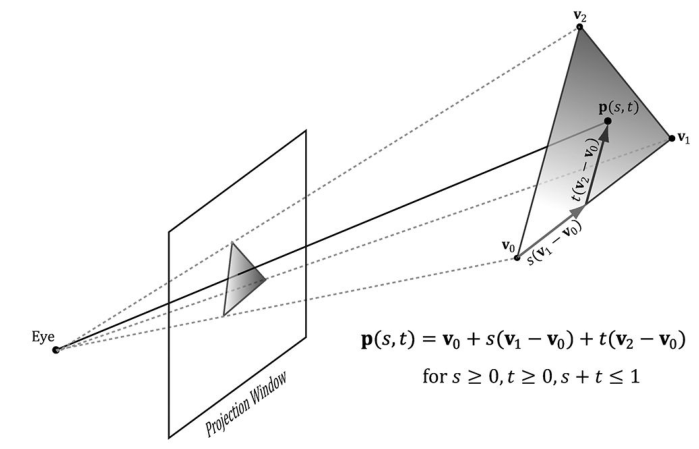
\includegraphics[width=\textwidth]{5-33}
    \centering
    \caption{通过对三角形顶点之间的属性值进行线性插值,可以得到三角形表面上的任一属性值p(s,t)。}
    \label{fig:5-33}
\end{figure}
\begin{flushleft}
我们不必关心透视精确插值的数学细节,因为硬件会自动完成这一工作;不过,有兴趣的读者可以在[Eberly01]中查阅相关的数学推导过程。图5.34介绍了一点基本思路:
\end{flushleft}
\begin{figure}[h]
    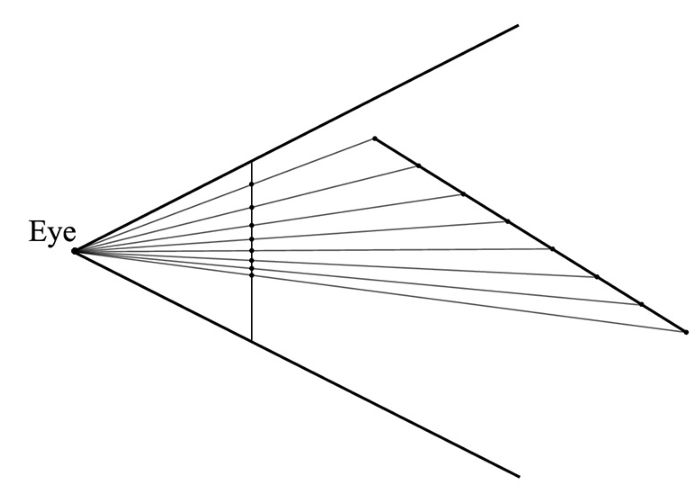
\includegraphics[width=\textwidth]{5-34}
    \centering
    \caption{一条3D线被投影到投影窗口上(在屏幕空间中投影是一条2D线)。我们看到,在3D线上取等距离的点,在2D屏幕空间上的投影点却不是等距离的。所以,我们在3D空间中执行线性插值,在屏幕空间需要执行非线性插值。}
    \label{fig:5-34}
\end{figure}

\section{像素着色器阶段(The Pixel Shader Stage)}
\begin{flushleft}
像素着色器(Pixel shader)是由我们编写的在GPU上执行的程序。像素着色器会处理每个像素片段(pixel fragment),它的输入是插值后的顶点属性,由此计算出一个颜色。像素着色器可以非常简单地输出一个颜色,也可以很复杂,例如实现逐像素光照、反射和阴影等效果。
\end{flushleft}
\section{输出合并阶段(The Output Merger Stage)}
\begin{flushleft}
当像素片段由像素着色器生成之后,它们会被传送到渲染管线的输出合并(output
merger,简称OM)阶段。在该阶段中,某些像素片段会被丢弃(例如,未能通过深度测试或模板测试)。未丢弃的像素片段会被写入后台缓冲区。混合(blending)工作是在该阶段中完成的,一个像素可以与后台缓冲区中的当前像素进行混合,并以混合后的值作为该像素的最终颜色。某些特殊效果,比如透明度,就是通过混合来实现的;我们会在第10章专门讲解混合。
\end{flushleft}

\chapter{在Direct3D中绘制(Drawing in Direct3D)}
\begin{flushleft}
在前一章中,我们主要关注渲染管线的概念和数学方面。 本章反过来关注配置渲染管道,定义顶点和像素着色器以及将几何图形提交到渲染管道进行绘制所需的Direct3D API接口和方法。 到本章结束时,您将能够绘制出具有纯色的3D框或线框模式。\\
~\\
{\large Objectives:}
\begin{itemize}
    \item 发现用于定义,存储和绘制几何数据的Direct3D接口方法。
    \item 学习如何写一个基本顶点和像素着色器
    \item 了解如何用管线状态对象配置渲染管线
    \item 理解如何创建和绑定缓冲数据常量到管线中,并且熟悉根签名
\end{itemize}
\end{flushleft}
\section{定点和顶点布局(Vertices and Input Layouts)}
\begin{flushleft}
5.5.1节已经讲过,在Direct3D中,顶点由空间位置和各种附加属性组成,Direct3D可以让我们灵活地建立属于我们自己的顶点格式;换句话说,它允许我们定义顶点的分量。要创建一个自定义的顶点格式,我们必须先创建一个包含顶点数据的结构体。例如,下面是两种不同类型的顶点格式;一个由位置和颜色组成,另一个由位置、法线和纹理坐标组成。
\end{flushleft}
\begin{lstlisting}
struct Vertex1
{
    XMFLOAT3 Pos;
    XMFLOAT4 Color;
}
struct Vertex2
{
    XMFLOAT3 Pos;
    XMFLOAT3 Normal;
    XMFLOAT2 Tex0;
    XMFLOAT2 Tex1;
}
\end{lstlisting}
\begin{flushleft}
我们定义好顶点构造体后,需要对该定点构造体进行描述然后提供给 Direct3D,让它知道如何去处理每个分量。此描述以D3D12\_INPUT\_LAYOUT\_DESC结构表示的输入布局描述(input layout description)的形式提供给Direct3D:
\begin{lstlisting}
typedef struct D3D12_INPUT_LAYOUT_DESC
{
    const D3D12_INPUT_ELEMENT_DESC *pInputElementDescs;
    UINT NumElements;
} D3D12_INPUT_LAYOUT_DESC;
\end{lstlisting}
一个输入布局描述就是一个简单的 D3D12\_INPUT\_ELEMENT\_DESC 元素数组和元素的数量。\\
~\\
D3D12\_INPUT\_ELEMENT\_DESC数组中的每个元素描述了对应的顶点结构体的分量。如果顶点构造体有两个分量,则对应的 D3D12\_INPUT\_ELEMENT\_DESC数组就有2个元素。D3D12\_INPUT\_ELEMENT\_DESC 定义如下:
\begin{lstlisting}
typedef struct D3D12_INPUT_ELEMENT_DESC
{
    LPCSTR SemanticName;
    UINT SemanticIndex;
    DXGI_FORMAT Format;
    UINT InputSlot;
    UINT AlignedByteOffset;
    D3D12_INPUT_CLASSIFICATION InputSlotClass;
    UINT InstanceDataStepRate;
} D3D12_INPUT_ELEMENT_DESC;
\end{lstlisting}
1. SemanticName: 一个与元素相关的字符串。它可以是任何有效的语义名。语义(semantic)用于将顶点结构体中的元素映射为顶点着色器参数(参见图\ref{fig:6-1})。\\
\begin{figure}[h]
    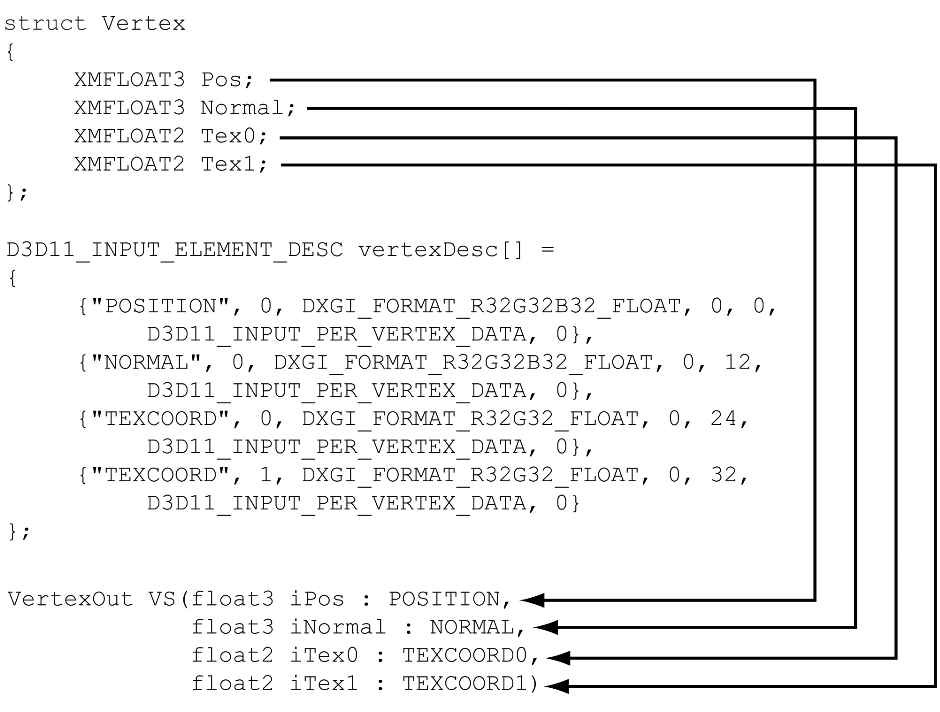
\includegraphics[width=\textwidth]{6-1}
    \centering
    \caption{顶点结构体中的每个元素分别由D3D11\_INPUT\_ELEMENT\_DESC数组中的对应元素描述。语义名和语义索引提供了一种将顶点元素映射为顶点着色器参数的方法。}
    \label{fig:6-1}
\end{figure}
2. SemanticIndex:附加在语义上的索引值。图\ref{fig:6-1}说明了使用该索引的原因;举例来说,当顶点结构体包含多组纹理坐标时,我们不是添加一个新的语义名,而是在语义名的后面加上一个索引值。在着色器代码中没有指定索引的语义默认索引为0,例如,在图\ref{fig:6-1}中的POSITION相当于POSITION0。\\
3. Format:一个用于指定元素格式的DXGI\_FORMAT枚举类型成员;下面是一些常用的格式:
\begin{lstlisting}
DXGI_FORMAT_R32_FLOAT          // 1D 32-bit float scalar
DXGI_FORMAT_R32G32_FLOAT       // 2D 32-bit float vector
DXGI_FORMAT_R32G32B32_FLOAT    // 3D 32-bit float vector
DXGI_FORMAT_R32G32B32A32_FLOAT // 4D 32-bit float vector
DXGI_FORMAT_R8_UINT            // 1D 8-bit unsigned integer scalar
DXGI_FORMAT_R16G16_SINT        // 2D 16-bit signed integer vector
DXGI_FORMAT_R32G32B32_UINT     // 3D 32-bit unsigned integer vector
DXGI_FORMAT_R8G8B8A8_SINT      // 4D 8-bit signed integer vector
DXGI_FORMAT_R8G8B8A8_UINT      // 4D 8-bit unsigned integer vector
\end{lstlisting}
4. InputSlot:指定当前元素来自于哪个输入槽(input slot)。Direct3D支持16个输入槽(索引依次为 0到15),通过这些输入槽我们可以向Direct3D传入顶点数据。例如,当一个顶点由位置元素和颜色元素组成时,我们既可以使用一个输入槽传送两种元素,也可以将两种元素分开,使用第一个输入槽传送顶点元素,使用第二个输入槽传送颜色元素。Direct3D可以将来自于不同输入槽的元素重新组合为顶点。在本书中,我们只使用一个输入槽,但是在本章结尾的练习2中我们会引导读者做一个使用两个输入槽的练习。\\
5. AlignedByteOffset:对于单个输入槽来说,该参数表示从顶点结构体的起始位置到顶点元素的起始位置之间的字节偏移量。例如在下面的顶点结构体中,元素Pos的字节偏移量为0,因为它的起始位置与顶点结构体的起始位置相同;元素Normal的字节偏移量为12,因为必须跳过由Pos占用的字节才能到达Normal的起始位置;元素Tex0的字节偏移量为24,因为必须跳过由Pos和Normal占用的字节才能到达Tex0的起始位置;元素Tex1的字节偏移量为32,因为必须跳过由Pos,Normal和Tex0占用的字节才能到达Tex1的起始位置。\\
\begin{lstlisting}
struct Vertex2
{
    XMFLOAT3 Pos;     // 0-byte offset
    XMFLOAT3 Normal;  // 12-byte offset
    XMFLOAT2 Tex0;    // 24-byte offset
    XMFLOAT2 Tex1;    // 32-byte offset
}
\end{lstlisting}
6. InputSlotClass:目前指定为D3D12\_INPUT\_PER\_VERTEX\_DATA;其他选项用于高级实例技术。\\
7. InstanceDataStepRate:目前指定为0;其他值只用于高级实例技术。\\
~\\
对于前面的两个示例顶点结构体Vertex1和Vertex2来说,对应的输入布局描述为:
\begin{lstlisting}
D3D12_INPUT_ELEMENT_DESC desc1[] = 
{
    {"POSITION", 0, DXGI_FORMAT_R32G32B32_FLOAT, 0, 0, D3D12_INPUT_PRE_VERTEX_DATA, 0},
    {"COLOR", 0, DXGI_FORMAT_R32G32B32A32_FLOAT, 0, 12, D3D12_INPUT_PRE_VERTEX_DATA, 0}
};
D3D12_INPUT_ELEMENT_DESC desc2[] =
{
    {"POSITION", 0, DXGI_FORMAT_R32G32B32_FLOAT, 0, 0,  D3D12_INPUT_PRE_VERTEX_DATA, 0},
    {"NORMAL", 0, DXGI_FORMAT_R32G32B32_FLOAT, 0, 12, D3D12_INPUT_PRE_VERTEX_DATA, 0},
    {"TEXCOORD", 0, DXGI_FORMAT_R32G32_FLOAT, 0, 24, D3D12_INPUT_PRE_VERTEX_DATA, 0},
    {"TEXCOORD", 1, DXGI_FORMAT_R32G32_FLOAT, 0, 32, D3D12_INPUT_PRE_VERTEX_DATA, 0}
};
\end{lstlisting}
\end{flushleft}
\section{顶点缓冲(Vertex Buffers)}
\begin{flushleft}
为了让GPU访问顶点数组,我们必须把它放置在一个称为缓冲(buffer)的GPU资源容器中, 我们称存储顶点的缓冲区叫顶点缓冲区。 缓冲区比纹理资源简单; 它们不是多维的,并且没有mipmap,过滤器或多采样支持。 无论何时我们需要为GPU提供一系列数据元素(如顶点),我们都会使用缓冲区。\\
~\\
就像4.3.8节一样,我们通过填充一个 D3D12\_RESOURCE\_DESC结构体来创建一个 ID3D12Resource 对象,并将其作为缓冲区资源。然后调用 ID3D12Device::CreateCommitedResource 方法。D3D12\_RESOURCE\_DESC 成员详情见 4.3.8 节。Direct3D 12 提供一个 C++ 包装类 CD3DX12\_RESOURCE\_DESC,它是 D3D12\_RESOURCE\_DESC 的衍生类,提供了方便的构造函数和方法。特别是,它提供了以下方法来简化描述缓冲区的D3D12\_RESOURCE\_DESC的构造:
\begin{lstlisting}
static inline CD3DX12_RESOURCE_DESC Buffer(
    UINT64 width, 
    D3D12_RESOURCE_FLAGS flags = D3D12_RESOURCE_FLAG_NONE,
    UINT64 alignment = 0)
{
    return CD3DX12_RESOURCE_DESC(D3D12_RESOURCE_DIMENSION_BUFFER, 
            alignment, width, 1, 1, 1, 
            DXGI_FORMAT_UNKNOWN, 1, 0,
            D3D12_TEXTURE_LAYOUT_ROW_MAJOR, flags);
}
\end{lstlisting}
对于一个缓冲区,width 相当于缓冲区的字节数。例,如果一个缓冲区存储64个浮点型(float),则 width 就是 64*sizeof(float)。\\
~\\
NOTICE: CD3DX12\_RESOURCE\_DESC类还提供了其他针对纹理资源和查询资源的方法:\\
\begin{itemize}
    \item 1. CD3DX12\_RESOURCE\_DESC::Tex1D
    \item 2. CD3DX12\_RESOURCE\_DESC::Tex2D
    \item 3. CD3DX12\_RESOURCE\_DESC::Tex3D
\end{itemize}
~\\
NOTICE:回忆第4章深度/模板缓冲区(depth/stencil buffer),这一阶段用ID3D12Resource 来表现 2D 纹理。所有在 Direct3D 12 的资源都用 ID3D12Resource 接口来表示。着和 Direct3D 11 中使用不同的接口表示不同的资源相反,像 ID3D11Buffer,ID3D11Texture2D。资源类型由 D3D12\_RESOURCE\_DESC::D3D12\_RESOURCE\_DIMENSION 属性指定。例:缓冲区有 D3D12\_RESOURCE\_DIMENSION\_BUFFER 和 2D 纹理 D3D12\_RESOURCE\_DIMENSION\_TEXTURE2D。\\
~\\
对于常量几何(不以每帧为基础改变的几何图形),我们将顶点缓冲区(vertex buffer)放入默认堆(D3D12\_HEAP\_TYPE\_DEFAULT)中,以提升性能。通常,一个游戏中大多数几何图形都是常量集合,像树、建筑、地形、人物等。顶点缓冲区初始化之后,只有GPU需要从顶点缓冲区中读取并画几何图形,所以默认堆就变得有意义了。然而,如果CPU不能将顶点缓冲区写入到默认堆中,我们如何才能初始化顶点缓冲区呢?\\
~\\
另外要新建实际的缓冲区资源,我们需要用D3D12\_HEAP\_TYPE\_UPLOAD新建一个中间上传缓冲资源。回忆4.3.8节,当我们需要从CPU到GPU复制数据时,我们将一个资源提交到上传队中。在创建上传缓冲区之后,从系统内存中复制顶点数据到上传缓冲区,然后从上唇缓冲区复制顶点数据到实际的顶点缓冲区中。\\
~\\
因为一个中间上传缓冲区需要初始化数据后的默认缓冲区(D3D12\_HEAP\_TYPE\_DEFAULT),所以为了代码重用性 d3dUtil.h/cpp 中建立了下面工具方法:
\begin{lstlisting}
Microsoft::WRL::ComPtr<ID3D12Resource> d3dUtil::CreateDefaultBuffer(
    ID3D12Device* device,
    ID3D12GraphicsCommandList* cmdList,
    const void* initData,
    UINT64 byteSize,
    Microsoft::WRL::ComPtr<ID3D12Resource>& uploadBuffer)
{
ComPtr<ID3D12Resource> defaultBuffer;

    // Create the actual default buffer resource.
    ThrowIfFailed(device->CreateCommittedResource(
        &CD3DX12_HEAP_PROPERTIES(D3D12_HEAP_TYPE_DEFAULT),
        D3D12_HEAP_FLAG_NONE,
        &CD3DX12_RESOURCE_DESC::Buffer(byteSize),
        D3D12_RESOURCE_STATE_COMMON,
        nullptr,
        IID_PPV_ARGS(defaultBuffer.GetAddressOf())));

    // In order to copy CPU memory data into our default buffer, we need to create
    // an intermediate upload heap. 
    ThrowIfFailed(device->CreateCommittedResource(
        &CD3DX12_HEAP_PROPERTIES(D3D12_HEAP_TYPE_UPLOAD),
        D3D12_HEAP_FLAG_NONE,
        &CD3DX12_RESOURCE_DESC::Buffer(byteSize),
        D3D12_RESOURCE_STATE_GENERIC_READ,
        nullptr,
        IID_PPV_ARGS(uploadBuffer.GetAddressOf())));

    // Describe the data we want to copy into the default buffer.
    D3D12_SUBRESOURCE_DATA subResourceData = {};
    subResourceData.pData = initData;
    subResourceData.RowPitch = byteSize;
    subResourceData.SlicePitch = subResourceData.RowPitch;

    // Schedule to copy the data to the default buffer resource.  
    // At a high level, the helper function UpdateSubresources
    // will copy the CPU memory into the intermediate upload heap.  
    // Then, using ID3D12CommandList::CopySubresourceRegion,
    // the intermediate upload heap data will be copied to mBuffer.
    cmdList->ResourceBarrier(1, &CD3DX12_RESOURCE_BARRIER::Transition(defaultBuffer.Get(), 
        D3D12_RESOURCE_STATE_COMMON, D3D12_RESOURCE_STATE_COPY_DEST));
    UpdateSubresources<1>(cmdList, defaultBuffer.Get(), uploadBuffer.Get(), 0, 0, 1, &subResourceData);
    cmdList->ResourceBarrier(1, &CD3DX12_RESOURCE_BARRIER::Transition(defaultBuffer.Get(),
        D3D12_RESOURCE_STATE_COPY_DEST, D3D12_RESOURCE_STATE_GENERIC_READ));

    // Note: uploadBuffer has to be kept alive after the above function calls because
    // the command list has not been executed yet that performs the actual copy.
    // The caller can Release the uploadBuffer after it knows the copy has been executed.
    return defaultBuffer;
}
\end{lstlisting}
D3D12\_SUBRESOURCE\_DATA 结构体定义如下:\\
\begin{lstlisting}
typedef struct D3D12_SUBRESOURCE_DATA
{
    const void *pData;
    LONG_PTR RowPitch;
    LONG_PTR SlicePitch;
} D3D12_SUBRESOURCE_DATA;
\end{lstlisting}
1. pData: 指向系统内存数组的指针,该系统内存数组包含了初始化缓冲区所需要的数据。如果缓冲区能保存 n 个顶点,则系统内存数组必须包含至少 n 个顶点的空间,以此来初始化整个缓冲区。\\
2. RowPitch:对于缓冲区,数据复制的字节大小。\\
3. SlicePitch:对于缓冲区,数据复制的字节大小。\\
~\\
下面代码展示了如何该类如何用于创建一个8顶点立方体的默认缓冲区,并且各个定点颜色不同:\\
\begin{lstlisting}
Vertex vertices[] = 
{
    {XMFLOAT3(-1.0f, -1.0f, -1.0f), XMFLOAT4(Colors::White)},
    {XMFLOAT3(-1.0f, +1.0f, -1.0f), XMFLOAT4(Colors::Black)},
    {XMFLOAT3(+1.0f, +1.0f, -1.0f), XMFLOAT4(Colors::Red)},
    {XMFLOAT3(+1.0f, -1.0f, -1.0f), XMFLOAT4(Colors::Green)},
    {XMFLOAT3(-1.0f, -1.0f, +1.0f), XMFLOAT4(Colors::Blue)},
    {XMFLOAT3(-1.0f, +1.0f, +1.0f), XMFLOAT4(Colors::Yellow)},
    {XMFLOAT3(+1.0f, +1.0f, +1.0f), XMFLOAT4(Colors::Cyan)},
    {XMFLOAT3(+1.0f, -1.0f, +1.0f), XMFLOAT4(Colors::Magenta)}
};
const UINT64 vbByteSize = 8 * sizeof(Vertex);
ComPtr<ID3D12Resource> VertexBufferGPU = nullptr;
ComPtr<ID3D12Resource> VertexBufferUploader = nullptr;
VertexBufferGPU = d3dUtil::CreateDefaultBuffer(
    md3dDevice.Get(),
    mCommandList.Get(),
    vertices, vbByteSize,
    VertexBufferUploader);
\end{lstlisting}
Vertex 类型定义如下:\\
\begin{lstlisting}
struct Vertex
{
    XMFLOAT3 Pos;
    XMFLOAT4 Color;
}
\end{lstlisting}
为了将顶点缓冲区绑定到管道,我们需要为顶点缓冲区资源创建一个顶点缓冲区视图(vertex buffer view)。不像一个RTV(render target view),我们不需要一个针对顶点缓冲区视图的描述堆(descriptor heap)。一个顶点缓冲区视图由 D3D12\_VERTEX\_BUFFER\_VIEW\_DESC 结构体表示:\\
\begin{lstlisting}
typedef struct D3D12_VERTEX_BUFFER_VIEW
{
    D3D12_GPU_VIRTUAL_ADDRESS BufferLocation;
    UINT SizeInBytes;
    UINT StrideInBytes;
} D3D12_VERTEX_BUFFER_VIEW;
\end{lstlisting}
1. BufferLocation:创建一个视图所需要的顶点缓冲区资源的虚拟地址。我们可以使用 ID3D12Resource::GetGPUVirtualAddress 方法获得该值。\\
2. SizeInBytes:从BufferLocation开始在顶点缓冲区中查看的字节数。 \\
3. StrideInBytes:每个顶点元素的字节大小。\\
在顶点缓冲区创建之后,我们再创建它的视图,我们能将其绑定到管道(pipeline)的一个输入槽(input slot),给输入汇编程序阶段(input assembler stage)提供顶点数据。使用下面方法就能做到:\\
\begin{lstlisting}
void ID3D12GraphicsCommandList::IASetVertexBuffers(
    UINT StartSlot,
    UINT NumBuffer,
    const D3D12_VERTEX_BUFFER_VIEW *pViews);
\end{lstlisting}
1. StartSlot:绑定顶点缓冲区的开始输入槽。共16个输入槽,0-15。\\
2. NumBuffers:绑定到输入槽的顶点缓冲区个数。如果开始槽索引为k,绑定了 n 个缓冲区,则绑定缓冲区的输入槽分别是$I_{k},I_{k}+1,...,I_{k}+n-1$。\\
3. pViews:指向顶点缓冲区视图数组的第一个元素的指针。\\
调用例子:\\
\begin{lstlisting}
D3D12_VERTEX_BUFFER_VIEW vbv;
vbv.BufferLocation = VertexBufferGPU->GetGPUVirtualAddress();
vbv.StrideInBytes = sizeof(Vertex);
vbv.SizeInBytes = 8 * sizeof(Vertex);
D3D12_VERTEX_BUFFER_VIEW vertexBuffers[1] = {vbv};
mCommandList->IASetVertexBuffers(0, 1, vertexBuffers);
\end{lstlisting}
IASetVertexBuffers 方法可能看起来有点复杂,因为它支持一个顶点缓冲区数组设置到不同的输入槽。然而,我们只使用一个输入槽。本章结尾会有练习,让你使用两个输入槽。\\
一个顶点缓冲区将保持绑定到输入插槽,直到您更改为止。 因此,如果您使用多个顶点缓冲区,则可以像这样构造代码:\\
\begin{lstlisting}
ID3D12Resource* mVB1; // stores vertices of type Vertex1
ID3D12Resource* mVB2; // stores vertices of type Vertex2
D3D12_VERTEX_BUFFER_VIEW_DESC mVBView1; // view to mVB1
D3D12_VERTEX_BUFFER_VIEW_DESC mVBView2; // view to mVB2

/*...Create the vertex buffers and views...*/
mCommandList->IASetVertexBuffers(0, 1, &VBView1);
/*...draw objects using vertex buffer 1...*/

mCommandList->IASetVertexBuffers(0, 1, &mVBView2);
/*...draw objects using vertex buffer 2...*/
\end{lstlisting}
给输入槽设置顶点缓冲区并不意味着绘制它们;这一步只是给管道提供顶点数据。最后一步才是绘制顶点,使用 ID3D12GraphicsCommandList::DrawInstanced 方法:\\
\begin{lstlisting}
void ID3D12GraphicsCommandList::DrawInstanced(
    UINT VertexCountPerInstance,
    UINT InstanceCount,
    UINT StartVertexLocation,
    UINT StartInstanceLocation);
\end{lstlisting}
1. VertexCountPerInstance:绘制顶点的数量(每个实例)。\\
2. InstanceCount:用于称为实例的高级技术; 现在,将其设置为1,因为我们只绘制一个实例。\\
3. StartVertexLocation:指定开始绘制的顶点缓冲区中第一个顶点的索引(从零开始)。\\
4. StartInstanceLocation:用于称为实例的高级技术; 现在,将其设置为0。\\
VertexCountPerInstance和StartVertexLocation这两个参数定义要绘制的顶点缓冲区中的顶点的连续子集;见图\ref{fig:6-2}。\\
\begin{figure}[h]
    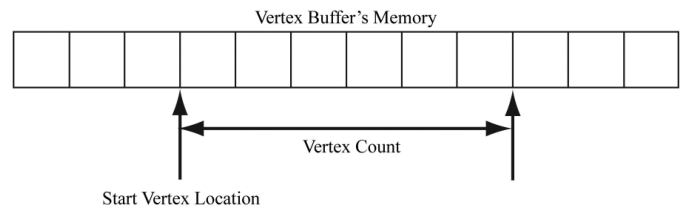
\includegraphics[width=\textwidth]{6-2}
    \centering
    \caption{StartVertexLocation 表示开始绘制的顶点缓冲区的第一个元素。VertexCountPerInstance 表示绘制顶点的个数。}
    \label{fig:6-2}
\end{figure}

DrawInstanced 方法没有制定顶点的基本类型。它们需要被绘制成点,线列表,还是三角列表?回忆5.5.2节,基本拓扑状态是通过 ID3D12GraphicsCommandList::IASetPrimitiveTopology 方法设置的。例:\\
\begin{lstlisting}
mCommandList->IASetPrimitiveTopology(D3D_PRIMITIVE_TOPOLOGY_TRIANGLELIST);
\end{lstlisting}
\end{flushleft}
\section{索引和索引缓冲区(Indices and Index Buffers)}
\begin{flushleft}
与顶点类似,为了让GPU访问索引数组,需要将索引数组放到GPU缓冲区资源中(ID3D12Resource)。我们将存储索引的缓冲区叫索引缓冲区(index buffer)。因为 d3dUtil::CreateDefaultBuffer 方法能通过 void* 作用于一般数据,我们同样使用该方法来创建索引缓冲区(或任何默认缓冲区)。\\
为了将索引缓冲区绑定到管道,我们需要为索引缓冲区资源创建一个索引缓冲区视图。 与顶点缓冲区视图一样,我们不需要一个描述符堆用于索引缓冲区视图。 索引缓冲区视图由D3D12\_INDEX\_BUFFER\_VIEW结构表示:\\
\begin{lstlisting}
typedef struct D3D12_INDEX_BUFFER_VIEW
{
    D3D12_GPU_VIRTUAL_ADDRESS bufferLocation;
    UINT SizeInBytes;
    DXGI_FORMAT Format;
} D3D12_INDEX_BUFFER_VIEW;
\end{lstlisting}
1. BufferLocation: 创建视图的顶点缓冲区资源的虚拟地址。 我们可以使用ID3D12Resource :: GetGPUVirtualAddress方法来获取它。\\
2. SizeInBytes:从BufferLocation开始在索引缓冲区中查看的字节数。\\
3. Format:索引的格式必须是16位索引的 DXGI\_FORMAT\_R16\_UINT 或32位索引的 DXGI\_FORMAT\_R32\_UINT。 如果索引值需要额外的32位范围,则应使用16位索引来减少内存和带宽,并仅使用32位索引。\\
~\\
就顶点缓冲区和其他Direct3D资源而言,在我们可以使用它之前,我们需要将它绑定到管道。 使用 ID3D12CommandList::SetIndexBuffer方法将索引缓冲区绑定到输入汇编程序阶段。 以下代码显示了如何创建一个定义多维数据集三角形的索引缓冲区,创建一个视图并将其绑定到管道:\\
\begin{lstlisting}
std::uint16_t indices[] = {
    // front face
    0, 1, 2,
    0, 2, 3,
    
    // back face
    4, 6, 5,
    4, 7, 6,
    
    // left face
    4, 6, 1,
    4, 1, 0,
    
    // right face
    3, 2, 6,
    3, 6, 7,
    
    // top face
    1, 5, 6,
    1, 6, 2,
    
    // bottom face
    4, 0, 3,
    4, 3, 7
};

const UINT ibByteSize = 36 * sizeof(std::uint16_t);

ComPtr<ID3D12Resource> IndexBufferGPU = nullptr;
ComPtr<ID3D12Resource> IndexBufferUploader = nullptr;
IndexBufferGPU = d3dUtil::CreateDefaultBuffer(md3dDevice.Get(), mCommandList.Get(), indices, ibByteSize, IndexBufferUploader);
D3D12_INDEX_BUFFER_VIEW ibv;
ibv.BufferLocation = IndexBufferGPU->GetGPUVirtualAddress();
ibv.Format = DXGI_FORMAT_R16_UINT;
ibv.SizeInBytes = ibByteSize;

mCommandList->IASetIndexBuffer(&ibv);
\end{lstlisting}
最后,使用索引时,用 ID3D12GraphicsCommandList::DrawIndexedInstanced 方法,而不是 DrawInstanced:\\
\begin{lstlisting}
void ID3D12GraphicsCommandList::DrawIndexedInstanced(
    UINT IndexCountPerInstance,
    UINT InstanceCount,
    UINT StartIndexLocation,
    INT BaseVertexLocation,
    UINT StartInstanceLocation);
\end{lstlisting}
1. IndexCountPerInstance:要绘制的索引数量(每个实例)。\\
2. InstanceCount:用于称为实例的高级技术; 现在,将其设置为1,因为我们只绘制一个实例。\\
3. StartIndexLocation:索引缓冲区中的一个元素索引,标志着开始读取索引的起始点。\\
4. BaseVertexLocation:在获取顶点之前,要将此整数值添加到此绘图调用使用的索引中。\\
5. StartInstanceLocation:用于称为实例的高级技术, 目前指定为0。\\
~\\
为了说明这些参数,请考虑以下情况。假设我们有三个对象:一个球体,一个盒子和一个圆柱体。首先,每个对象都有自己的顶点缓冲区和自己的索引缓冲区。每个本地索引缓冲区中的索引都与相应的本地顶点缓冲区有关。现在假设我们将球体,盒子和圆柱体的顶点和索引连接成一个全局顶点和索引缓冲区,如图\ref{fig:6-3}所示。 (可能会连接顶点和索引缓冲区,因为在更改顶点和索引缓冲区时会有一些API开销,这很可能不是瓶颈,但是如果有许多小的顶点和索引缓冲区可以很容易地合并,值得这样做是出于性能方面的原因。)在这个串联之后,索引不再是正确的,因为它们存储索引位置相对于它们相应的本地顶点缓冲区而不是全局索引位置;因此需要重新计算索引以正确地将索引指向全局顶点缓冲区。原始盒子索引是在假设盒子的顶点贯穿索引的情况下计算出来的 0, 1, ..., numBoxVertices-1\\
但是合并之后,就成为:\\
\begin{lstlisting}
firstBoxVertexPos,
firstBoxVertexPos+1,
...,
firstBoxVertexPos+numBoxVertices-1
\end{lstlisting}
 
\begin{figure}[h]
    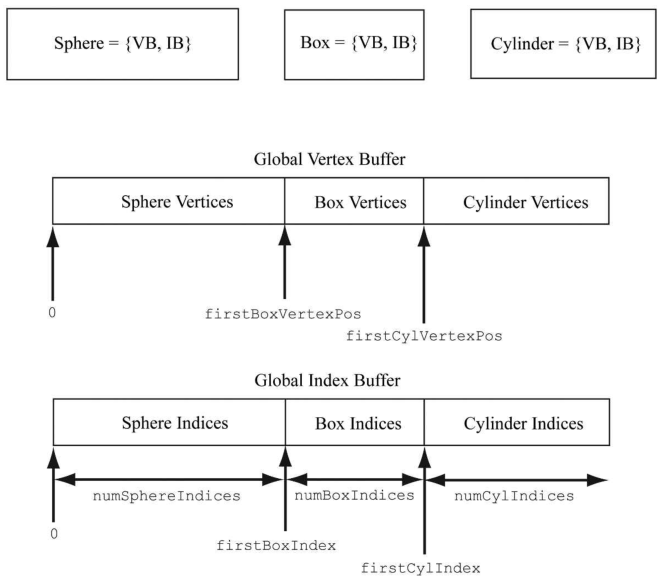
\includegraphics[width=\textwidth]{6-3}
    \centering
    \caption{将几个顶点缓冲区连接成一个大的顶点缓冲区,并将几个索引缓冲区连接成一个大的索引缓冲区。}
    \label{fig:6-3}
\end{figure}

因此,要更新索引,我们需要为每个框索引添加第一个BoxVertexPos。 同样,我们需要为每个柱面索引添加firstCylVertexPos。 请注意,球体的指标不需要改变(因为第一个球体顶点位置为零)。 让我们把对象的第一个顶点相对于全局顶点缓冲区的位置称为它的基本顶点位置。 通常,对象的新索引是通过将其基本顶点位置添加到每个索引来计算的。 我们可以让Direct3D通过将基本顶点位置传递给DrawIndexedInstanced的第四个参数来完成它,而不必自己计算新的索引。\\
然后我们可以用以下三个调用一个接一个地绘制球体,盒子和圆柱体:\\
\begin{lstlisting}
mCmdList->DrawIndexedInstanced(numSphereIndices, 1, 0, 0, 0);
mCmdList->DrawIndexedInstanced(numBoxIndices, 1, firstBoxIndex, firstBoxVertexPos, 0);
mCmdList->DrawIndexedInstanced(numCylIndices, 1, firstCylIndex, firstCylVertexPos, 0);
\end{lstlisting}
下一章(chapter)"Shapse"代码样例就使用了这样的技术。
\end{flushleft}
\section{顶点着色器例子(Example Vertex Shader)}
TODO
\section{像素着色器例子(Example Pixel Shader)}
TODO
\section{常量缓冲区(Constant Buffers)}
\subsection{创建常量缓冲区(Creating Constant Buffers)}
\begin{flushleft}
常量缓冲区是GPU资源(ID3D12Resource)的一个例子,其数据内容可在着色器程序中引用。 正如我们将在本书中学习的那样,着色器程序中也可以引用纹理和其他类型的缓冲区资源。 6.4节中的示例顶点着色器的代码如下:
\begin{lstlisting}
cbuffer cbPerObject: register(b0)
{
    float4x4 gWorldViewProj;
}
\end{lstlisting}
此代码引用一个名为cbPerObject的cbuffer对象(常量缓冲区)。 在这个例子中,常量缓冲区存储一个名为gWorldViewProj的4×4矩阵,表示用于将点从本地空间转换为同类剪辑空间的组合世界,视图和投影矩阵。 在HLSL中,4×4矩阵由内置的float4x4类型声明; 要声明3×4矩阵和2×4矩阵,例如,您将分别使用float3x4和float2x2类型。\\
与顶点和索引缓冲区不同,常量缓冲区通常由CPU每帧更新一次。 例如,如果摄像机每帧移动一次,则每帧必须使用新的视图矩阵更新常量缓冲区。 因此,我们在上传堆而不是默认堆中创建常量缓冲区,以便我们可以从CPU更新内容。\\
常量缓冲区也有特殊的硬件要求,它们的大小必须是最小硬件分配大小(256字节)的倍数。\\
通常我们需要多个相同类型的常量缓冲区。 例如,上面的常量缓冲区cbPerObject存储每个对象不同的常量,所以如果我们有n个对象,那么我们将需要n个这种类型的常量缓冲区。 以下代码显示了我们如何创建一个存储NumElements多个常量缓冲区的缓冲区:
\begin{lstlisting}
struct ObjectConstants
{
    DirectX::XMFLOAT4X4 WorldViewProj = MathHelper::Identity4x4();
};
UINT elementByteSize = d3dUtil::CalcConstantBufferByteSize(sizeof(ObjectConstants));
ComPtr<ID3D12Resource> mUploadCBuffer;
device->CreateCommittedResource(
    &CB3DX12_HEAP_PROPERTIES(D3D12_HEAP_TYPE_UPLOAD), 
    D3D12_HEAP_FLAG_NONE, 
    &CD3DX12_RESOURCE_DESC::Buffer(elementByteSize * NumElements),
    D3D12_RESOURCE_STATE_GENERIC_READ,
    nullptr, 
    IID_PPV_ARGS(&mUploadCBuffer));
\end{lstlisting}
我们可以将mUploadCBuffer视为存储ObjectConstants类型的常量缓冲区数组(使用填充为256的倍数)。 当需要绘制一个对象时,我们只需将一个常量缓冲区视图(CBV)绑定到缓冲区的一个存储该对象常量的子区域。 请注意,我们经常会调用缓冲区mUploadCBuffer作为常量缓冲区,因为它存储了一个常量缓冲区数组。\\
工具函数 d3dUtil::CalcConstantBufferByteSize 会进行算术运算将缓冲区的字节大小舍入为最小硬件分配大小(256字节)的倍数:\\
\begin{lstlisting}
static UINT CalcConstantBufferByteSize(UINT byteSize)
{
    // Constant buffers must be a multiple of the minimum hardware
    // allocation size (usually 256 bytes).  So round up to nearest
    // multiple of 256.  We do this by adding 255 and then masking off
    // the lower 2 bytes which store all bits < 256.
    // Example: Suppose byteSize = 300.
    // (300 + 255) & ~255
    // 555 & ~255
    // 0x022B & ~0x00ff
    // 0x022B & 0xff00
    // 0x0200
    // 512
    return (byteSize + 255) & ~255;
}
\end{lstlisting}
NOTICE: 即使我们以256的倍数分配常量数据,也不需要在HLSL结构中明确填充相应的常量数据,因为它是隐式完成的:\\
\begin{lstlisting}
// Implicitly padded to 256 bytes.
cbuffer cbPerObject : register(b0)
{
    float4x4 gWorldViewProj;
};

// Explicitly padded to 256 bytes.
cbuffer cbPerObject : register(b0)
{
    float4x4 gWorldViewProj;
    float4x4 Pad0;
    float4x4 Pad1;
    float4x4 Pad1;
}
\end{lstlisting}
NOTICE: 为避免处理将常量缓冲区元素舍入为256字节的倍数,可以明确地将所有常量缓冲区结构填充为256字节的整数倍。\\
~\\
Direct3D 12推出了着色器模型5.1。 Shader model 5.1引入了一种替代HLSL语法来定义一个常量缓冲区,如下所示:\\
\begin{lstlisting}
struct ObjectConstants
{
    float4x4 gWorldViewProj;
    uint matIndex;
};
ConstantBuffer<ObjectConstants> gObjConstants : register(b0);
\end{lstlisting}
这里常量缓冲区的数据元素只是在一个单独的结构中定义,然后从该结构创建一个常量缓冲区。 然后使用数据成员语法在着色器中访问常量缓冲区的字段:\\
\begin{lstlisting}
uint index = gObjConstants.matIndex;
\end{lstlisting}
\end{flushleft}

\subsection{更新常量缓冲区(Updating Constant Buffers)}

\end{document}
